In questo capitolo verrà approfondito il processo di generazione codice del progetto Go e del manifest wadm, che verranno impiegati poi per le fasi di Build e Deploy. Il primo passo è definire con precisione le struttura e la composizione dei file che fanno parte del progetto iniziale, quello che dovrà poi configurare l'utente finale che utilizzerà il framework, strutturato nel modo seguente:

\texttt{project/}
\dirtree{%
.1 workflow.yaml.
.1 tasks/.
.2 task1.go.
.1 gen/.
}

\section{Definizione Tasks}

In questa sezione ci si concentrerà sulle specifiche dei file task, cioè quelli situati nella cartella \texttt{tasks} del progetto e contenenti le funzioni che verranno eseguite dai moduli Wasm. Iniziamo fornendo la struttura base di ogni task file, mostrata nel Listing \ref{code:task_file}.
\begin{lstlisting}[language=Go, caption={Struttura base file task}, captionpos=b, label={code:task_file}]
    package main
    import (
    	...
    )
    ...    
    func exec_task(arg string) string{
    
    	return ... 
    }
\end{lstlisting}

I requisiti da rispettare per la definizione della task sono:
\begin{itemize}
    \item Il file deve avere un'estensione \texttt{.go}.
    \item Il package deve essere impostato su main (stesso package del main fornito dal template).
    \item Funzione di interfacciamento (cioè chiamata dal main) nominata \texttt{exec\_task}.
    \item La funzione di interfacciamento deve accettare una stringa e restituire una stringa.
\end{itemize}

La funzione interfaccia accetta e restituisce una stringa per facilitare il più possibile l'utilizzo da parte di un utente finale, che non dovrà preoccuparsi di tradurre i tipi Go con i tipi Wasm specificati in WASI (cosa che viene gestita in ``background'' sul file main del progetto Go).\\
Una volta soddisfatti questi requisiti è possibile eseguire innumerevoli operazioni, come importare librerie, definire strutture e altre funzioni. Un esempio è mostrato nel Listing \ref{code:task_file_json}, in cui viene importata la libreria \texttt{encoding/json} e definita una struct \texttt{Request}.

\begin{lstlisting}[language=Go, caption={Task file ed integrazione con Json}, captionpos=b, label={code:task_file_json}, keepspaces=true]
    package main
    import (
        "encoding/json"
    )
    type Request struct {
        Data int
        Name string
    }
    func exec_task(arg string) string{
        // unmarshal the data
        req := Request{}
        json.Unmarshal([]byte(arg), &req)
    
        // do some operations
        ...
        
        // return the json string
        json, _ := json.Marshal(req)
        return string(json)
    }
\end{lstlisting}

\section{Configurazione Workflow}

Passiamo ora alla codifica del file \texttt{workflow.yaml}, nel quale verranno effettivamente impostati i task e il loro comportamento. 

\subsection{Specifica file workflow}

Il file deve essere correttamente formattato in Yaml e contenere i seguenti campi:
\begin{itemize}
    \item \texttt{project\_name}: stringa contenente il nome del progetto, può contenere spazi e viene utilizzato principalmente nella CLI e nelle metriche.
    \item \texttt{tasks}: lista contenente i vari componenti Wasm.
\end{itemize}

Andando nel dettaglio, ogni elemento della lista \texttt{tasks} deve contenere:
\begin{itemize}
    \item \texttt{name}: stringa contenente il nome del componente, può contenere spazi e verrà impostato come nome dell'applicazione su wasmCloud.
    \item \texttt{type}: stringa contenente il template da utilizzare come base.
    \item \texttt{code}: stringa contenente il nome del file task da associare al componente Wasm in fase di generazione.
    \item \texttt{targets}: lista contenente delle stringhe che rappresentano la label \texttt{host-type} associata ai nodi target di deployment dei componenti Wasm.
    \item \texttt{source\_topic}: stringa contenente il topic da cui verranno ricevuti i dati.
    \item \texttt{dest\_topic}: stringa contenente il topic a cui verranno inviati.
    \item \texttt{component\_name}: stringa contenente il nome sintetico del componente, non può contenere spazi e funge da nome per l'OCI artifact associato.
    \item \texttt{version}: versione del componente, specificata nel formato \texttt{x.x.x}. Insieme al component\_name conferisce il nome all'OCI artifact.
    
\end{itemize}

\subsection{Template}

I template sono dei progetti già sviluppati che forniscono certe funzionalità e fungono da base per il codice fornito dall'utente. Attualmente sono implementati due template:
\begin{itemize}
    \item \texttt{processor\_nats}: comunicazione interamente basata su NATS: i dati arrivano da un topic e vengono inviati ad un topic.
    \item \texttt{http\_producer\_nats}: i dati possono provenire sia da un topic NATS che da una richiesta POST effettuata al nodo in cui è deployata l'applicazione. Viene utilizzato infatti l'http provider per esporre un web server nella porta 8000.
\end{itemize}

Questo approccio consente una facile estendibilità del progetto: infatti potranno essere sviluppati ed aggiunti nuovi template per aumentare le funzionalità disponibili sul framework. Un altro template attualmente in sviluppo è quello per la scrittura dei dati su un DB relazionale.\\
Per comprendere meglio le modalità di utilizzo del file workflow analizziamo un esempio.

\begin{lstlisting}[language=yaml, caption={Esempio Workflow file con processor e producer}, captionpos=b, label={code:workflow_file}, keepspaces=true]
project_name: Temperature data analysis
tasks:
  - name: Temp data conversion
    type: http_producer_nats
    code: convert.go
    targets:
      - edge
    source_topic: living_room_celsius_data
    dest_topic: living_room_kelvin_data
    component_name: celsius_to_kelvin_conversion
    version: 1.0.0
  - name: Data filter
    type: processor_nats
    code: filter.go
    targets:
      - cloud
    source_topic: living_room_kelvin_data
    dest_topic: filtered_kelvin_data
    component_name: temp_filter
    version: 1.0.2
\end{lstlisting}

Nel file workflow riportato nel Listing \ref{code:workflow_file} vengono definiti due componenti:
\begin{itemize}
    \item il primo si occupa di ricevere dati inviati da sensori ad un server http, convertire le temperature e pubblicarli in un topic NATS
    \item il secondo filtra i risultati, magari rimuovendo errori di misurazione o aggregandoli
\end{itemize}
Questo semplice esempio vuole mostrare come con una configurazione ridotta sia possibile generare, compilare e distribuire un'applicazione che supporta casi d'uso applicabili al mondo IoT.

\section{Generazione codice}

Il codice che si occupa della generazione è situato sul package \texttt{code\_generator} ed è distribuito nei file \texttt{generator.py} e \texttt{template\_compiler.py}. All'interno del package sono presenti anche i template utilizzati come base per i progetti Go, situati nella cartella \texttt{templates}.
\texttt{code\_generator/}
\dirtree{%
.1 .
.1 generator.py.
.1 template\_compiler.py.
.1 templates/.
.2 processor\_nats/.
.2 producer\_nats/.
}

\subsection{Parsing Workflow}

Verrà ora analizzato nel dettaglio il processo di generazione del codice, partendo dalla fase di analisi del progetto fornito dall'utente. La prima operazione viene effettuata da \texttt{generator.py}, di cui riportiamo un estratto contenente il codice più rilevante.
\begin{lstlisting}[language=python, caption={Generazione del codice}, captionpos=b, label={code:code_gen}]
    def generate(project_dir, registry_url, metrics, metrics_enabled):
        ...
        # Parsing del file workflow.yaml
        config = __parse_yaml(f"{project_dir}/workflow.yaml")
        
        # Pulizia della cartella di output
        __remove_dir_if_exists(output_dir)
        os.makedirs(output_dir, exist_ok=True)
        
        # Per ogni task all'interno del file workflow
        for task in config['tasks']:
            ...
            # Compilazione dei template
            template_compiler.handle_task(task, output_dir)

            # Copia del file task all'interno della cartella di output
            shutil.copy2(f"{project_dir}/tasks/{task['code']}", f"{output_dir}/{task['component_name']}/{task['code']}")
                
        if metrics_enabled:
            gen_metrics['gen_time'] = '%.3f'%(end_time - start_time)
            metrics['code_gen'] = gen_metrics
\end{lstlisting}

Come si può notare dal Listing \ref{code:code_gen} la funzione \texttt{generate} si occupa di parsare il file workflow, controllarne la validità e preparare la cartella di output. 

\subsection{Compilazione template}

La generazione vera e propria del codice viene affidata a \texttt{template\_compiler} tramite la funzione \texttt{handle\_task}, la quale seleziona il template corretto in base a quello riportato nella configurazione, lo copia nella cartella di output e lo compila utilizzando Jinja.\\
Nei Listing \ref{code:jinja_after} e \ref{code:jinja_after} viene riportato un esempio di file (in questo caso una porzione di \texttt{wadm.yaml}) prima e dopo la compilazione del template tramite Jinja.\\

\noindent\begin{minipage}{.46\textwidth}
\begin{lstlisting}[caption=Template wadm.yaml, language=yaml, basicstyle=\scriptsize, frame=single, label={code:jinja_before}]
spec:
  components:
    - name: {{ component_name }}
      type: component
      properties:
        image: "{{ registry_url }}/{{ component_name }}:{{ version }}"
      traits:
        - type: link
          properties:
            target: nats-processor
            namespace: wasmcloud
            package: messaging
            interfaces: [consumer]
        - type: spreadscaler
          properties:
            instances: 1
            spread:
            
            
            - name: {{ target }}
              weight: {{ weight }}
              requirements:
                host-type: {{ target }}
            
\end{lstlisting}
\end{minipage}
\hfill
$\rightarrow$
\hfill
\begin{minipage}{.46\textwidth}
\begin{lstlisting}[caption=wadm.yaml compilato con Jinja, language=yaml, basicstyle=\scriptsize, frame=single, label={code:jinja_after}]
spec:
  components:
    - name: data_double_test1
      type: component
      properties:
        image: "gitea.rebus.ninja/lore/data_double_test1:1.0.0"
      traits:
        - type: link
          properties:
            target: nats-processor
            namespace: wasmcloud
            package: messaging
            interfaces: [consumer]
        - type: spreadscaler
          properties:
            instances: 1
            spread:
            - name: cloud
              weight: 100
              requirements:
                host-type: cloud
\end{lstlisting}
\end{minipage}

A questo punto viene copiato il file specificato sulla configurazione dalla cartella \texttt{task/} del progetto alla cartella di output. La funzione viene automaticamente agganciata all'handler specifico del file main del template (dato che appartengono allo stesso package).\\

L'intero processo di generazione è stato schematizzato nella Figura \ref{fig:code_gen_impl}:

\FloatBarrier
\begin{figure}[h]
    \centering
    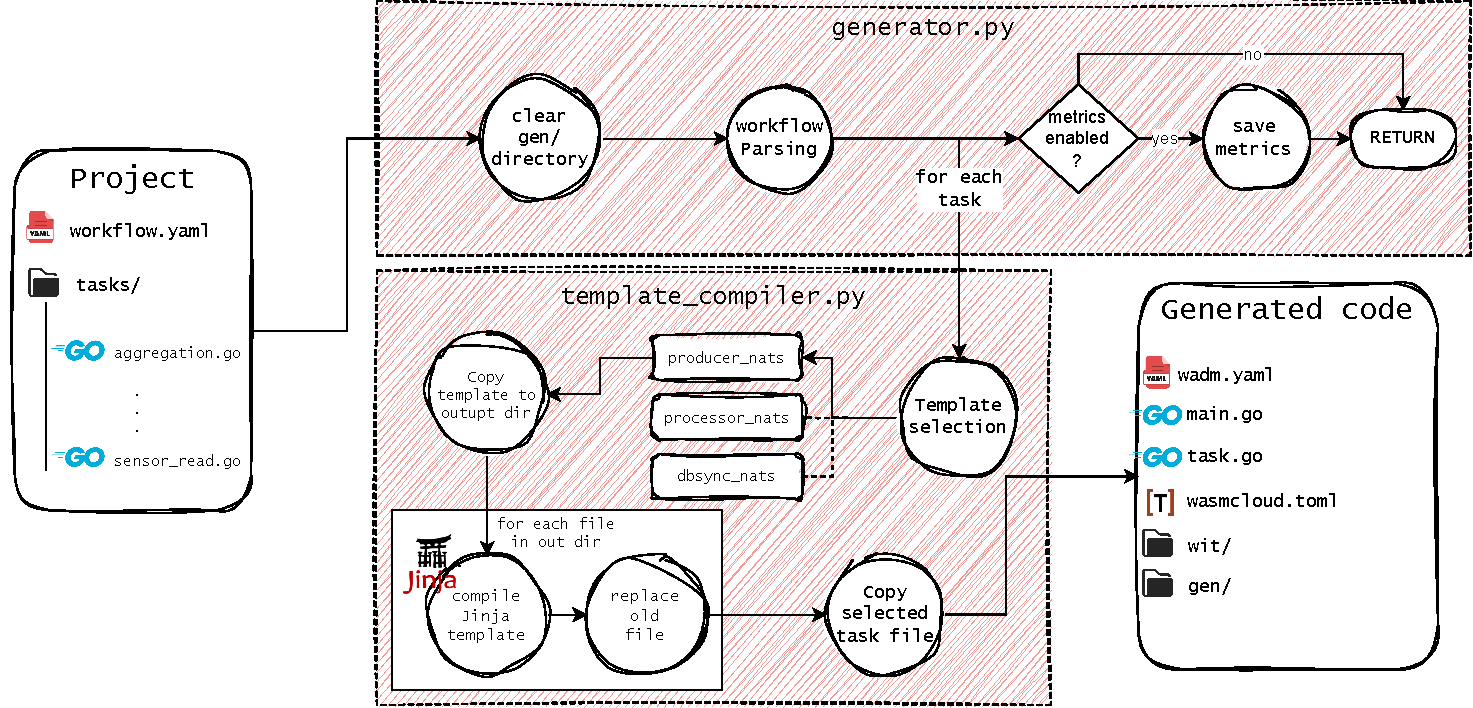
\includegraphics[width=\textwidth]{img/schemi/schemi-implementazione-gen.drawio.pdf}
    \caption{Processo generazione del codice}
    \label{fig:code_gen_impl}
\end{figure}
\FloatBarrier